\documentclass[a4paper,12pt]{report}
\usepackage{alltt, fancyvrb, url}
\usepackage{graphicx}
\usepackage[utf8]{inputenc}
\usepackage{hyperref}
\usepackage{setspace}
\usepackage{wrapfig}
\usepackage{xcolor}


% Questo commentalo se vuoi scrivere in inglese.
\usepackage[italian]{babel}

\usepackage[italian]{cleveref}

\title{Relazione:\break``DUKEMANIA''}

\author{Gianluca Migliarini, \\ Serafino Pandolfini,\\ Sofia Tosi,\\ Laura Leonardi, \\ Alessandro Brasini}
\date{25 Agosto 2021}

 
\begin{document}

\maketitle
\tableofcontents




\chapter{Analisi}
\section{Requisiti}
Il gruppo si pone come obbiettivo quello di realizzare un clone del videogioco musicale "BeatManiaIIDX".
Lo sviluppo mira alla completa funzionalità a livello di gameplay, e, in aggiunta all'opera originale
dalla quale viene presa ispirazione, offrire all'utente la possibilità di importare i propri livelli giocabili tramite file Midi (Musical Instrument Digital Interface). Viene inoltre considerato come requisito la sostituzione della riproduzione di una traccia audio con la sintesi sonora in tempo reale.
\subsubsection{Requisiti funzionali}
\begin{itemize}
	\item L'utente è in grado di scegliere quale canzone giocare a partire dalla scelta di un file Midi.
	\item L'applicativo deve riprodurre fedelmente tutte le tracce componenti la canzone, con un timbro musicale
	simile a quello di un GameBoy.
	\item L'applicativo deve offrire un gameplay su varie colonne, il giocatore dovrà premere le note sulla rispettiva colonna a ritmo di musica per ottenere punti.
	\item L'applicativo deve memorizzare una scoreboard con tutti i punteggi delle varie partite relative alla canzone selezionata.
	\item La traccia giocabile viene scelta dall'utente dalla lista delle tracce componenti la canzone.
	\item L'applicativo deve "semplificare" le traccie musicali complesse rendendole giocabili, segnalando un grado di difficoltà
\end{itemize}

\subsubsection{Requisiti non funzionali}
\begin{itemize}
	\item L'applicativo deve funzionare correttamente sia su Windows sia su sistemi basati su Unix
	\item La fluidità del gameplay e la qualità dell'audio non devono essere compromesse dalla pesantezza del file midi (ovviamente se non troppo complesso)
\end{itemize}
\newpage

% section analisi di modello e dominio
\section{Analisi e modello del dominio}


Dukemania dovrà essere in grado di fare selezionare all'utente il proprio nickname e una canzone in formato Midi. Dovrà inoltre permettere la configurazione dei nomi di tracce e strumenti associati alla canzone selezionata. Inoltre, la traccia da giocare, sara' anch'essa selezionabile dall'utente.
I vari strumenti saranno caricati a partire da un file di configurazione in locale all'avvio del gioco e saranno detti sintetizzatori.
Ci sarà una entità responsabile della gestione e riproduzione del tono e del volume in entrata e in uscita. Le tracce della canzone, con le relative note, verranno individuate da un parser. A ogni traccia verrà associato un solo sintetizzatore che riprodurrà uno strumento.
Il gameplay si svolgerà su varie colonne, in ognuna delle quali cadranno note relative alla traccia selezionata, opportunamente semplificata per garantirne la giocabilità.
Le difficoltà primarie riguarderanno il calcolo del punteggio in base alla precisione del giocatore e la sincronizzazione tra la caduta delle note e il suono riprodotto.
Alla fine della partita, dovrà essere visualizzata una schermata contenente il punteggio migliore di ogni singolo giocatore ottenuto sulla canzone selezionata in precedenza.
\begin{figure}[!htb]
	\centerline{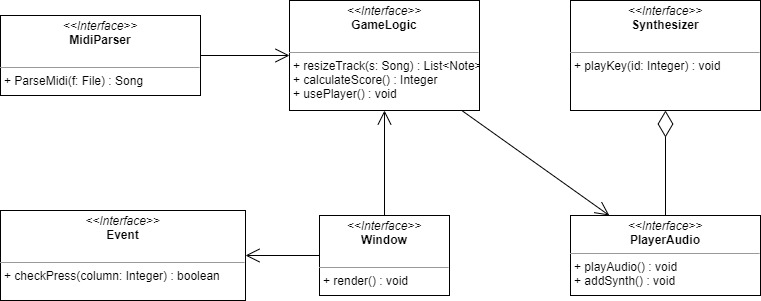
\includegraphics[scale=0.7]{img/uml_analisi.jpg}}
	\caption{Schema UML della fase di analisi.}
	\label{img:analysis}
\end{figure}
\newpage


\chapter{Design}
\section{Architettura}
L'architettura di DukeMania è basata sul pattern MVC.
La classe DukeMania è l'entry point dell'applicazione, al suo interno vengono inizializzate tutte le View e il WindowManager, la classe che fungerà da Controller principale.
Il compito pricipale di WindowManager è quello di cambiare, tra le varie View, la finestra da renderizzare e visualizzare, occupandosi inoltre di passare il Model alle varie schermate, che a loro volta lo passeranno al relativo Controller.
Il Model principale, rappresentato da GameModel, conterrà le configurazioni di gioco, rendendole così accessibili a tutte le View.
La classe WindowManager implementa l'interfaccia SwitchWindowNotifier, il cui compito principale e' quello di notificare il WindowManager, segnalandogli che un controller di una View vuole sostituire la finestra attiva.
Tutte le View implementano l'interfaccia Window, la quale le rende predisposte a ricevere i dati del Model, e ad utilizzare lo SwitchWindowNotifier tramite il proprio controller.
Utilizzando questa strategia è semplice aggiungere nuove View e definirne il comportamento.
\newpage
\section{Design dettagliato}
\subsection{Gianluca Migliarini}
La classe Engine si occupa di aggiornare e visualizzare lo stato dei vari sintetizzatori (tastiere simulate),
ad ogni chiamata del metodo render viene riempito un buffer di samples (campioni audio), ogni campione audio viene calcolato sommando i campioni audio di tutti i sintetizzatori al momento della chiamata.
Una volta che il buffer e' pieno, viene mandato al dispositivo audio che si occupa di suonare i vari campioni.
Ogni traccia della canzone viene suonata da un sintetizzatore, per differenziare i sintetizzatori delle percussioni da quelli di tastiere e' stata creata l' interfaccia Synth, contenente solamente i metodi comuni tra i due, ovvero quello per fermare le note/percussioni che hanno finito di suonare e quello per ottenere un sample da scrivere sub buffer audio in uscita. 
Le variabili di impostazioni che garantiscono il corretto funzionamento dell'audio sono scritte nella classe Settings.java, come campi finali statici.
TODO FACTORY SYNTH?
Per evitare costi computazionali troppo alti, i vari campioni delle varie note di tutti i sintetizzatori vengono pre-caricati in istanze anonime dell'interfaccia BufferManager, la quale estende l'interfaccia iterator, in quanto, oltre al nuovo metodo per ri-iniziare a suonare una nota/percussione (refresh), e' necessario avere metodi per controllare se un altro campione puo' essere riprodotto e per ottenere quest'utlimo.
\subsubsection{DrumSynth}
Nel caso del sintetizzatore per le percussioni, le varie istanze di BufferManager sono presenti come campo dell'enum DrumSamples. Ho scelto di utilizzare questo enum come pattern "singleton" in quanto non richiede l' istanziazione di oggetto, e perche' l'AudioEngine gira solamente su un Thread.
L'unico metodo esterno all'interfaccia Synth e' playPercussion, il quale si occupa di ri-iniziare la riproduzione di un elemento della batteria.
\subsubsection{KeyboardSynth}
Per i vari sintetizzatori di tastiere, oltre ai metodi dell'interaccia Synth, e' presente il metodo playTimeNote, per suonare una nota ad una determinata frequenza per un determinato tempo espresso in microsecondi. Inoltre, ad ogni Synth viene associato un Enveloper, per determinare il tempo di attacco e di caduta della nota, espressi in millisecondi. I BufferManager delle note vengono creati all'istanziamento del sintetizzatore seguendo calcoli che coinvolgono le onde che danno la forma al suono, anche queste gia' caricate in vettori read only in un enum singleton (WaveTable), al fine di ridurre i calcoli matematici.
A seconda dello strumento da simulare, le note possono seguire degli LFO, ovvero delle funzioni che cambiano lo il pitch e il volume della nota nel tempo, per la creazione di queste funzioni ho scelto di utilizzare il pattern "factory", in quanto il tipo e' lo stesso ma le implementazioni sono differenti.
Per impostare correttamente tutti i parametri dei sintetizzatori di tastiera ho inoltre utilizzato il pattern "builder".
Le note dei vari sintetizzatori vengono suonate da PlayerAudio, che periodicamente controllera' quando ad ogni nota arriva il suo tempo di essere suonata.
\newpage
\subsection{membro 2}
progetto 
\newpage
\subsection{Sofia Tosi}
Questo paragrafo illustra il design relativo alla gestione dell'input e degli assets.
In seguito ad un'attenta valutazione, il gruppo ha stabilito di far interfacciare l'utente all'applicazione DukeMania tramite l'utilizzo di
una tastiera per pc. 
Durante la progettazione della sezione concernente l'input, ho ritenuto oppurtuno utilizzare il pattern Adapter.
La classe EventsFromKeyboardImpl rappresenta l'Adapter in sè che, implementando l'interfaccia omonima, riesce a semplificare e a permettere l'interazione
tra la tastiera, che sfrutta la libreria com.badlogic.gdx.Input, e la classe relativa alla grafica PlayScreen.
Per non superare eccessivamente l'ammontare di ore, l'applicazione attuale è stata implementata per consentire solo l'utilizzo della tastiera del pc. 
Laddove si volesse, in futuro, cambiare la periferica, l'applicazione non esclude questa possibilità. Si potrebbe infatti implementare EventsFromKeyboard 
e sostituire la classe dell'adapter con un altro adapter che interagisca con una diversa periferica (ad esempio un gamepad, una SG Guitar Hero o una tastiera midi).
\\ \\
singleton \\
Un'altra peculiare classe che merita di essere citata è l'AssetManager che, come dice il nome si dedica all'organizzazione degli assets, ovvero tutte le risorse grafiche
necessarie per il corretto funzionamento dell'applicazione. Queste risorse, che possono essere, ad esempio, le texture degli elementi nella GUI o i file con i font utilizzati,
vengono caricate una sola volta in memoria.
Ho deciso di sfruttare il pattern Singleton per la realizzazione di tale classe. Difatti è importante che ci sia una sola istanza dell'AssetManager per evitare che le risorse 
grafiche vengano istanziate più volte in memoria sprecando spazio inutilmente. 
\newpage
\subsection{membro 4}
progetto 
\subsection{membro 5}
progetto 
\newpage



\chapter{Sviluppo}
\section{Testing}
test \\ \\
{\setstretch{0.6}
Le classi che sono state testate sono: \\
\begin{itemize}
	\item \textbf{LFO:} per ogni funzione LFO è presente un test per garantire il corretto funzionamento della funzione di ritorno della factory
	
	\item \textbf{KeyboardSynth:} testato la correttezza del conto di quante note stanno suonando al momento, il metodo per ottenere il campione audio, il metodo per risuonare una nota.
	
	\item \textbf{DrumSynth:} testato la correttezza del conto di quante percussioni stanno suonando al momento, il metodo per ottenere il campione audio, il metodo per risuonare una percussione.
	
	\item \textbf{SynthBuilder:} testate le eccezioni
\end{itemize}
}
\newpage
\section{Metodologia di lavoro}
\subsection{Gestione del lavoro}
Lo sviluppo del progetto è stato preceduto da una fase preliminare di analisi, durante la quale tutti insieme abbiamo lavorato per definire le basi dell'applicazione e, successivamente, per specificare i vari dettagli implementativi tramite UML.
La suddivisione delle parti del progetto è avvenuta in modo equo assegnando a ciascuno una parte significativa e importante del progetto.
\subsection*{Gestione del DVCS}
Per il DVCS è stato utilizzato git, in quanto è stato il Software spiegato a lezione. Abbiamo creato una repository su github e abbiamo deciso di creare un branch per ogni membro del team. In seguito, quando ritenuto che ognuno di noi avesse implementato il "core" della propria parte, abbiamo deciso di eseguire un merge in un nuovo branch "alpha", sul quale ogni membro ha continuato a salvare le proprie modifiche e sul quale sono stati effettuati i primi test di giocabilità.
\newpage

\subsection*{Suddivisione del lavoro}
\subsection{membro 1}
Sviluppo del Motore Audio, ideazione della gestione delle note, studi matematici per la rappresentazione di onde audio a partire da funzioni.
Gestione dei volumi delle note e delle percussioni, sviluppo di filtri e funzioni per garantire varietà tra i timbri sonori. \\ \\
Classi sviluppate singolarmente:
{\setstretch{0.6}
	\begin{itemize}
		\item DrumSamples
		\item DrumSynth
		\item Engine
		\item Enveloper
		\item Filters
		\item KeyboardSynth
		\item LFOFactory
		\item PlayerAudio
		\item Settings
		\item SynthBuilder
		\item WaveTable
	\end{itemize}
}
\hfill\break
\textbf{• Problematiche riscontrate}\hfill\break
problemi 
\newpage

\subsection{membro 2}
ha fatto questo bla bla bla \\ \\
Classi sviluppate singolarmente:
{\setstretch{0.6}
	\begin{itemize}
		\item classe 1
		\item classe 1
		\item classe 1
	\end{itemize}
}
\hfill\break
\textbf{• Problematiche riscontrate}\hfill\break
problemi 
\newpage

\subsection{Sofia Tosi}
In questa sezione si parlerà di grafica. La classe principale è PlayScreen, il cuore della View, attraverso la
quale vengono richiamate tutte le altre classi implementate dalla sottoscritta e alcune classi dei miei compagni. 
Questa classe, alla quale ho dedicato più tempo, mi ha messo alla prova e mi ha stimolato a voler conoscere cose nuove. Infatti per implementarla
mi sono servita della libreria grafica Libgdx, con la quale non avevo mai lavorato. Un'idea che mi è balenata in mente mentre la implementavo, che non si è 
manifestata durante l'analisi svolta all'inizio del progetto, è quella di creare una classe a parte, EventsFromKeyboard, 
per gestire i comandi di input. EventsFromKeyboard, come vuole suggerire il nome, è stata pensata per essere combatibile con una tastiera per pc. 
Nulla vieta di avvalersi di un'altra periferica. Infatti, ho cercato di limitare al massimo le dipendenze in PlayScreen in modo tale che risulti semplice sostituirla, 
avendo a disposizione un'altra classe compatibile con un'altra periferica.
Ho ritenuto opportuno implementare AssetManager per gestire le risorse grafiche. Questa classe permette di caricare in memoria tutte gli asset grafici in una
sola volta. Sarà poi il compito di PlayScreen richiamarli singolarmente, al momento opportuno, e mostrarli a video.
Tra i miei compagni del gruppo, quello con cui ho dovuto interagire di più è Serafino Pandolfini, ed è stato proprio da quest'interazione che è scaturita la classe
KeyImpl. Lo scopo di KeyImpl è proprio quello di fornirgli dei metodi per poter ottenere il tempo di inizio e di fine nel quale l'utente preme un tasto.
Una classe fondamentale da utilizzare in PlayScreen è NoteImpl. NoteImpl rappresenta la nota, ma a differenza del Notelogic(la nota logica) e il,
la rappresenta dal punto di vista grafico. In questa classe sono presenti i metodi per disegnare la nota, per disegnare le scintile che compaiono sulla nota quando l'utente la
preme al momento giusto. Nonostante sia una classe che implementa metodi legati alla grafica si è cercato di limitare il più possibile l'uso di libgdx, per ridurre il più
possibile le dipendenze. Un'ultima classe che merita di essere citata è senza dubbio SizeImpl, la quale adatta la GUI alla dimensione dello schermo del pc sul quale viene 
lanciata l'applicazione.
Per collaborare io e i miei compagni abbiamo deciso di stabilire insieme come dovevano essere strutturate le interfacce e successivamente abbiamo implementato il
codice basandoci sulle decisioni prese. Fortunatamente non ci sono stati particolari problemi, almeno per quanto riguarda la mia parte, e, in caso di dubbi, eravamo sempre disponibili
a confrontarci. \\ \\
Classi sviluppate singolarmente:
{\setstretch{0.6}
	\begin{itemize}
		\item PlayScreen
		\item AssetManager
		\item EventsFromKeyboard
		\item EventsFromKeyboardImpl
		\item Note
		\item NoteImpl
		\item Size
		\item SizeImpl
		\item Key
		\item KeyImpl
		\item ComputingShift
		\item ComputingShiftImpl
	\end{itemize}
}
\hfill\break
\textbf{• Problematiche riscontrate}\hfill\break
problemi 
\newpage

\subsection{membro 4}
ha fatto questo bla bla bla \\ \\
Classi sviluppate singolarmente:
{\setstretch{0.6}
	\begin{itemize}
		\item classe 1
		\item classe 1
		\item classe 1
	\end{itemize}
}
\hfill\break
\textbf{• Problematiche riscontrate}\hfill\break
problemi 
\newpage

\subsection{membro 5}
ha fatto questo bla bla bla \\ \\
Classi sviluppate singolarmente:
{\setstretch{0.6}
	\begin{itemize}
		\item classe 1
		\item classe 1
		\item classe 1
	\end{itemize}
}
\hfill\break
\textbf{• Problematiche riscontrate}\hfill\break
problemi 
\newpage



\section{Note di sviluppo}
schermata
\newpage

\subsection{Gianluca Migliarini}
Feature avanzate del linguaggio:
\begin{itemize}
	\item \textbf{lambda:} usate per caricare gli iteratori delle note per ogni traccia e i buffer dei campioni audio nei sintetizzatori di tastiere.
	\item \textbf{stream:} usati per controllare lo stato di tutti i sintetizzatori e sommare i vari campioni di questi ultimi.
	\item \textbf{optional:} usati per i campi opzionali nel builder dei sintetizzatori di tastiera. 
	\item \textbf{function:} usate per gestire gli LFO
\end{itemize}
Librerie utilizzate:
\begin{itemize}
	\item \textbf{libgdx:} utilizzata per Gdx.audio.newAudioDevice, necessario per riprodurre sul dispositivo audio hardware il buffer di campioni.
\end{itemize}
Classi riutilizzate: \\
Per comodità ho deciso di riutilizzare la classe generica Pair, introdotta dal prof. Viroli durante il corso.
\newpage

\subsection{membro 2}
commenti
\begin{itemize}
	\item \textbf{lambda:} tanta roba
	\item \textbf{stream:} tanta roba
\end{itemize}
librerie utilizzate:
\begin{itemize}
	\item \textbf{libgdx:} gestione grafica
\end{itemize}
\newpage

\subsection{Sofia Tosi}
commenti
\begin{itemize}
	\item \textbf{lambda:} tanta roba
	\item \textbf{stream:} tanta roba
\end{itemize}
librerie utilizzate:
\begin{itemize}
	\item \textbf{libgdx:} libreria grafica Libgdx: studio autonomo di tale libreria per realizzare l'interfaccia di gioco.
\end{itemize}
Classi riutilizzate: \\
Utilizzo della classe Pair fornita gentilmente dal professore Viroli
\newpage

\subsection{membro 4}
commenti
\begin{itemize}
	\item \textbf{lambda:} tanta roba
	\item \textbf{stream:} tanta roba
\end{itemize}
librerie utilizzate:
\begin{itemize}
	\item \textbf{libgdx:} gestione grafica
\end{itemize}
\newpage

\subsection{membro 5}
commenti
\begin{itemize}
	\item \textbf{lambda:} tanta roba
	\item \textbf{stream:} tanta roba
\end{itemize}
librerie utilizzate:
\begin{itemize}
	\item \textbf{libgdx:} gestione grafica
\end{itemize}
\newpage




\chapter{Commenti Finali}
\section{Autovalutazione e lavori futuri} \\
schermata 
\newpage

\section{Gianluca Migliarini}
\subsection{commenti}
Sono molto soddisfatto del gruppo e del lavoro che siamo riusciti a portare a termine.
Essendo una delle mie prime esperienze di lavoro in team ho trovato delle difficoltà principalmente riguardanti
la gestione del tempo e a volte la coordinazione con gli altri membri, per questo ringrazio i miei compagni per la disponibilità e per aver tenuto sempre un clima sereno durante lo sviluppo; ritengo quindi che questo progetto mi abbia permesso di crescere notevolmente dal punto di vista organizzativo, in particolare per l'utilizzo di un software per la gestione del versioning.
Inoltre sono molto felice di essere riuscito ad inserire in un progetto concreto il mio interesse per la sintesi audio.
\subsection{difficoltà riscontrate}
In conclusione, ritengo che il corso sia stato più che sufficiente per garantirmi uno sviluppo del progetto senza problematiche troppo grandi a livello implementativo, e che mi abbia incentivato ad utilizzare gli aspetto più avanzati del linguaggio, i quali avrei probabilmente evitato.
\newpage
\section{Serafino Pandolfini}
\subsection{commenti}
Sono personalmente soddisfatto del lavoro che ho svolto; fin dai miei primi approcci alla programmazione ho sempre preferito, piuttosto che dedicarmi a particolari funzionalità di librerie, a porre il mio interesse sulle strutture dati e le loro organizzazioni e in questo progetto ho avuto modo di mettermi alla prova in un contesto che non fosse il mio solito programma giocattolo scoprendo le mie effettive conoscenze e capacità. Ho avuto modo di apprezzare in particolare gli stream e le loro funzionalità che riuscivano sempre a stupirmi. È stata ricorrente la situazione in cui emergeva un problema ed esisteva già un operazione in grado di risolverlo in modo quasi istantaneo.
Non ho intenzione di continuare a sviluppare questo progetto ma se non mi fossi limitato al monte ore richiesto mi sarebbe piaciuto sviluppare altre modalità di gioco con calcoli dei punteggi e gameplay differenti prendendo ispirazione da altri giochi simili. 
\subsection{difficoltà riscontrate}
Il progetto non è stato esente da difficoltà, principalmente la coordinazione tra i vari membri per quanto ottimale ha portato a incomprensioni sul funzionamento di certi aspetti e talvolta si è dovuto ricorrere a soluzioni non ottimali dal mio punto di vista. Dal mio punto di vista però l'emergere di queste difficoltà mi ha permesso di avere una comprensione più completa del progetto che non avrei avuto altrimenti.
\newpage
\section{Sofia Tosi}
\subsection{commenti}
DukeMania è stato il mio primo grande progetto a cui ho preso parte. 
Non nego la mia preoccupazione iniziale, poi però pian piano durante l'analisi e implementando codice è svanita.
Questo progetto mi ha permesso di crescere ampiamente, in vari ambiti.
In primo luogo, ho imparato cosa significa scrivere codice di qualità e a quanto siano importanti i pattern.
Al contempo, ho anche aumentato la mia conoscenza studiando una nuova libreria grafica e conoscendo meglio le potenzialità di Git e LaTex. 
Realizzare DukeMania non è stato affatto facile, soprattutto perchè si tratta di un gioco musicale e le mie conoscenze musicali
sono esigue. Ma grazie alla collaborazione con i miei compagni, tutti molto disponibili e gentili siamo riusciti nel nostro intento.
Indipendentemente dalla valutazione finale, mi ritengo molto soddisfatta del progetto.
\subsection{difficoltà riscontrate}
Ritengo il corso di Programmazione ad Oggetti un corso molto valido e interessante. 
Mi ha permesso di approfondire nuovi argomenti non soltanto da autodidatta, ma anche con le lezioni dei prof 
che le ho trovate chiare e stimolanti. L'unica modifica che apporterei è l'aggiunta di ore di laboratorio per
imparare già da subito a prendere la mano con i pattern e Csharp. Nella mia modesta opinione avere più ore da dedicare a questi argomenti
comporterebbe un notevole aiuto.
\newpage
\section{Laura Leonardi}
\subsection{commenti}
progetto 
\subsection{difficoltà riscontrate}
progetto 
\newpage

\section{Alessandro Brasini}
\subsection{commenti}
Tenendo in conto degli ostacoli incontrati nel corso dello sviluppo del progetto per arrivare a conoscere libgdx, mi sento molto soddisfatto del risultato finale ottenuto.
Sono inoltre riconoscente ai miei compagni di team, i quali hanno mantenuto un approccio serio e professionale, nonostante la nostra comune inesperienza riguardante il lavoro in gruppo.
Ho imparato l'importanza della fase di ideazione del progetto e l'utilità di suddividere equamente, tra compagni, il carico di lavoro, senza mai sottovalutare l'importanza di un DVCS, il quale si è rivelato fondamentale.
In conclusione, la cosa che ho imparato di più da questo progetto, è il programmare in una modalità più responsabile e consapevole, in quanto i miei collaboratori riponevano fiducia nel mio lavoro come io nel loro.
\subsection{difficoltà riscontrate}
Durante il mio percorso formativo avevo già avuto occasione di programmare ad oggetti, ma è stato solamente dopo questo corso che ho capito la vera utilità di concetti come interfacce e classi astratte. Inoltre sono grato di aver utilizzato java, in quanto ho avuto la possibilità di imparare a programmare in un linguaggio del tutto nuovo, e per la prima volta ricco di sfaccettature e funzioni avanzate.
Ritengo infine che le uniche problematiche inerenti al corso siano dovute dalla metodologia di lezione a distanza, problemi che purtroppo si sono riversati durante gli appelli d'esame e che mi hanno impedito di beneficiare degli insegnamenti al massimo.
\newpage

\chapter{Appendice}
Guida Utente: \\


\end{document}